\documentclass[11pt,a4paper]{article}
\usepackage[margin=24mm]{geometry}
\usepackage[T1]{fontenc}
\usepackage[utf8]{inputenc}
\usepackage{lmodern,microtype,amsmath,amssymb,booktabs,graphicx,natbib,hyperref}
\hypersetup{colorlinks=true,linkcolor=blue,citecolor=blue,urlcolor=blue}
\setlength{\parskip}{4pt}
\setlength{\parindent}{0pt}
\setlength{\belowcaptionskip}{5pt}
\title{Learning when additional spectral measurements improve mango dry-matter estimates across harvest seasons}
\author{Author names and affiliations: author input required}
\date{Author-review manuscript; software replay study}
\begin{document}
\maketitle
\begin{abstract}
A partial optical scan can be inaccurate either because useful installed channels remain unread or because the installed bank cannot recover information available to a richer spectrum. We evaluate whether teaching this distinction improves sequential mango dry-matter prediction. The study uses 10,243 development scans from three seasons and separately evaluates 1,448 and 320 scans from two later seasons. Ten digitized manufacturer emitter profiles support selection of an eight-channel bank with two initial measurements. Group-cross-fitted assay errors provide bank-completion and next-channel targets; a matched alternative learns its stopping target against a rich-spectrum reference. Disjoint harvest populations support bank design, fitting and calibration. Operating points target four mean development readings and are frozen before external scoring. In season 4, the two-reference and single-reference controllers had RMSEP 2.672 and 2.752 pp, with 3.096 and 2.365 mean readings, respectively. In season 5, the two-reference and single-reference controllers had RMSEP 1.997 and 2.171 pp, with 4.809 and 2.369 mean readings, respectively. The illustrative prototype criteria did not hold in both seasons. Measurements are simulated finite-band responses, harvest populations substitute for unavailable fruit identifiers, and earlier local work reused the external benchmarks. The study evaluates empirical value rather than claiming a new general early-exit principle or physically validated scanner.
\end{abstract}

\section{Introduction}
Near-infrared measurements offer an indirect estimate of mango dry matter, but season, cultivar, temperature and instrument variation complicate transfer. Selecting a small optical bank and deciding how much of that bank to read are distinct problems. A stopping rule that compares a partial prediction with a rich-spectrum model can encourage acquisition even when the installed bank cannot deliver the missing information. Conversely, an accurate complete bank does not imply that its useful corrections are predictable from an early scan.

This study asks two questions. First, does a controller trained on assay-relative improvement from completing its installed bank improve on an otherwise matched controller trained against a rich-spectrum reference? Second, do the resulting error--acquisition trade-offs meet explicitly illustrative engineering criteria for a prototype? Negative and inconclusive results answer these questions without establishing hardware feasibility.

\subsection{Related work and contribution boundary}
Finite-response mango filter design already combines simulated optical responses with supervised prediction and filter selection \citep{gutierrez2019}. Seasonal calibration robustness, robust modeling, CNN benchmarking, augmentation with variable selection, multiscale ensembles, and L1-selected SVR are relevant mango precedents \citep{anderson2020,mishra2023,walsh2024,yang2025,yang2026,ma2026}. Their published scores cannot be ranked against the present split as if they were local matched experiments. Full methods were inaccessible for six journal leads; the source audit explicitly separates bibliographic and partial-text verification from full-text review.

Conditional spectral acquisition predates this work \citep{huang2015}. Dynamic feature selection learns expected predictive-loss reductions \citep{covert2023}; non-greedy acquisition can optimize over future subsets \citep{valancius2024}. Supervised early-exit risk already compares early and full-model losses \citep{jazbec2024}. BAARC also studies adaptive spectral acquisition and uncertainty-based stopping \citep{baarc2026}. Thus neither learned stopping, adaptive spectroscopy nor the basic loss-gap concept is new here. The narrow empirical contribution tested is separating bank-correctable error from the bank's excess error against a richer spectral model in a seasonal mango evaluation. No claim of absolute originality or patentability follows from this comparison.

\section{Materials and methods}
\subsection{Public data, observation unit and split}
We use the original CSV from Mendeley Data version 3, DOI 10.17632/46htwnp833.3 \citep{andersondata2024}. The download matches the provider's SHA-256. The official version-4 listing supplies the same version-3 content; the expanded multi-instrument data are not counted as independent replication. The complete CSV contains 12,011 scans. Seasons 1--3 contain 3,914, 1,363 and 4,966 scans from 25, 19 and 50 harvest populations. Seasons 4 and 5 contain 1,448 and 320 scans from 18 and 2 populations. The outcome is laboratory dry matter as percent of fresh weight; prediction errors are percentage points (pp).

There is no verified row-level fruit identifier. Provider guidance describes repeated scans, including temperature repeats. We therefore group by documented harvest population nested within season and do not infer fruit identities from equal assays. Unique fruit counts remain unknown. Metadata provide cultivar, region, date and temperature categories, but not a calibrated exact temperature or instrument serial identifier per row. No exact common-grid spectral duplicate sets were found within or across seasons. The raw CSV spans 285--1200 nm; the comparison uses exactly 103 channels from 684 to 990 nm at 3-nm increments. Provider page descriptions disagree with the raw extent, which is documented in the audit.

Each outer development fold holds out one whole season. Of the remaining harvest populations, 20\% are reserved for calibration. From the remaining pool, 15\% are reserved solely for supervised bank construction. All fitting and inner target cross-fitting exclude these bank-design and calibration populations. The final deployment fit repeats this scheme on seasons 1--3. Seeds and complete row/group assignments are saved. An independent pre-external code audit identified the need for the separate bank-design subset; preliminary attempts were retained and affected fits rerun. Neither external season informed that repair.

Earlier local work evaluated the same later-season benchmarks. We did not consult its numerical results for this analysis, but disclose the reuse and do not characterize these data as a newly collected, untouched independent replication.

\subsection{Optical response model}
Ten distinct eligible real-part profiles were digitized from typical Roithner emitter plots \citep{roithnercatalog}. The catalog preserves part identifiers, source PDFs, plot coordinates, traced curves, nominal bandwidths, support coverage and checksums. Eight LEDs are installed; both endpoint channels in the bank are read initially and charged. The instrument manual describes apparent absorbance as Log(1/Reflectance), but does not explicitly state the log base. We use the conventional base-10 interpretation and retain this unresolved instrument-specific qualification.

For apparent absorbance $A_i$, relative intensity is $r_i=10^{-A_i}$. With emitter response, assumed detector/reference response and bin widths combined into $w_{ji}$, the emulated normalized channel is
\begin{equation}
z_j=-\log_{10}\left(\frac{\sum_i w_{ji}10^{-A_i}}{\sum_i w_{ji}}\right).
\end{equation}
A flat detector/reference response is assumed because a calibrated curve is unavailable. At least 95\% of modeled profile mass must lie within the comparison window. A constant-spectrum invariant is tested. Sparse inference uses only requested channel values and masks; no full-spectrum normalization, derivatives or interpolation appears in the deployed predictor. Gaussian profiles based on nominal center/FWHM, center shifts and width perturbations are separately labeled sensitivities. These channels are simulations of typical curves, not measured device responses. Pulse counts represent acquisition effort; no joule, optical SNR or physical scan-time result is claimed.

\begin{figure}[tb]
\centering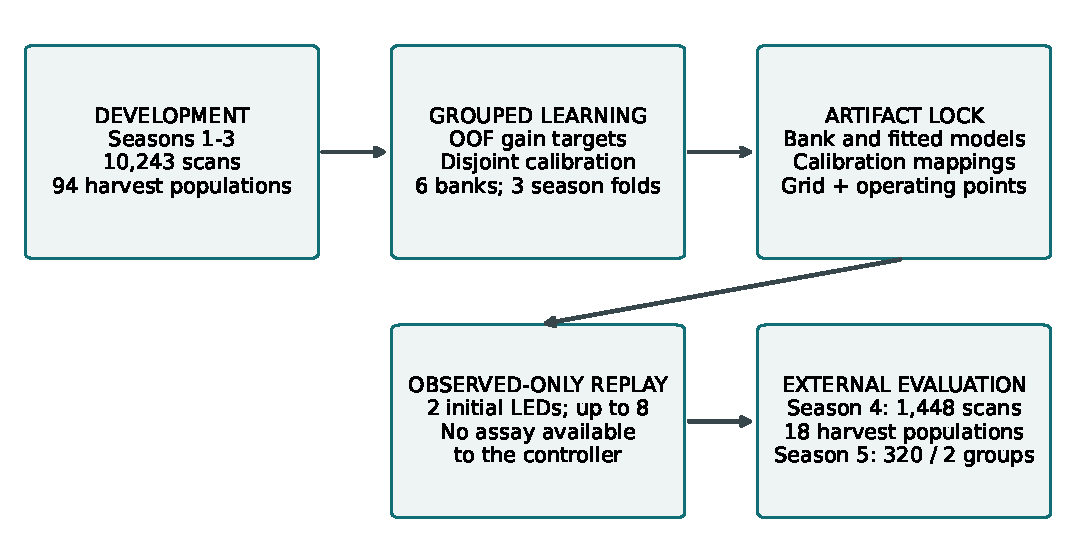
\includegraphics[width=\linewidth]{../figures/study_design.pdf}
\caption{Registered information boundaries. Harvest populations remain together; all models and operating points are frozen before external assays enter the evaluator.}
\end{figure}
\begin{figure}[tb]
\centering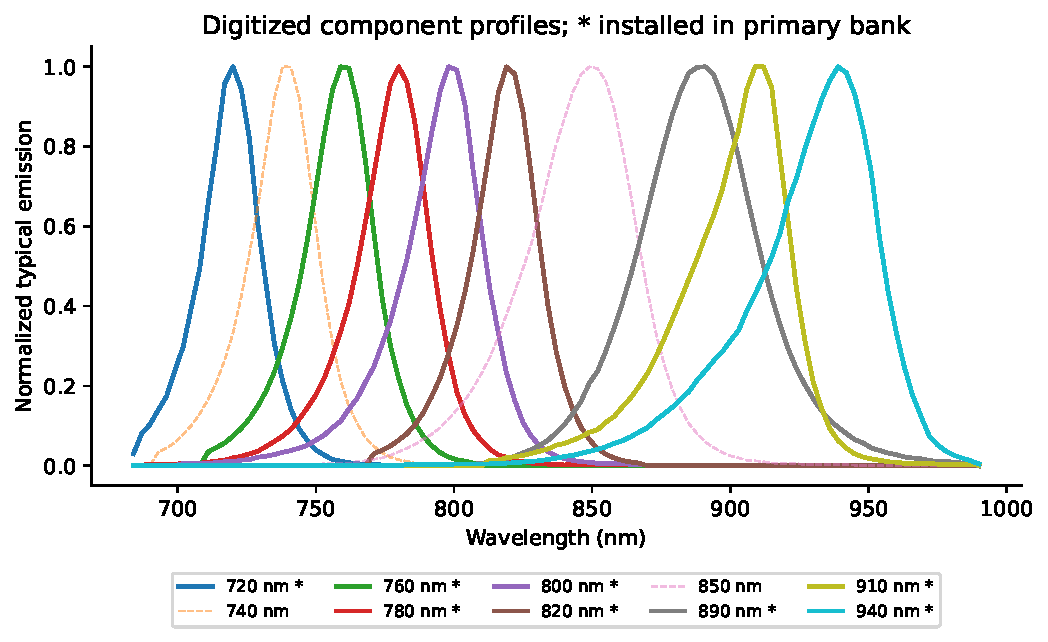
\includegraphics[width=\linewidth]{../figures/led_profiles.pdf}
\caption{Digitized typical emission profiles and the selected bank. Actual detector response and device-to-device variation require physical validation.}
\end{figure}

\subsection{Predictors and controller targets}
Let $f_S$, $f_B$ and $f_F$ predict the same assay $y$ from an acquired subset, the installed bank, and the rich spectrum. Write $e_U=|y-f_U|$. We distinguish
\begin{align}
g_{\mathrm{stop}}&=e_S-e_B,\\
g_{\mathrm{bank}}&=e_B-e_F,\\
g_j&=e_S-e_{S\cup\{j\}}.
\end{align}
Negative gains are retained. A material correction is $g>0.50$ pp; descriptive sensitivities use 0.25 and 1.00 pp. This is an illustrative engineering threshold, not a verified grower requirement. Bank losses combine information and model-fitting differences; neither reference is ground truth.

A masked MLP takes standardized acquired readings and a binary mask through hidden layers of 64 and 32 units. An unread standardized value is replaced by zero independently of its true value. Acquired zero is distinguished by its mask. Three group-disjoint inner folds generate partial and reference predictions for controller targets. A frozen six-component PLS bank predictor is used both in its targets and at the all-installed endpoint, making the endpoint stop gain exactly zero. The rich PLS reference uses row SNV, an 11-point second derivative and 12 components. Such full-spectrum transformations are confined to this offline reference.

The controller has the same 64/32 hidden architecture, a binary probability head, signed next-action scores and an auxiliary residual-error head. BCE and standardized signed-gain MSE receive equal weight; residual MSE has weight 0.25. The proposed binary label is $g_{\mathrm{stop}}>0.50$; the matched alternative uses $e_S-e_F>0.50$. Action targets, initialization, training masks, effort and bank are matched. We enumerate all 64 masks reachable from the two initial channels for out-of-fold target prediction, using the 63 nonterminal masks to train the controller. Each scan has equal total mask weight. Probability calibration uses disjoint calibration-population sequential paths. At runtime, continue with the highest-scored unread LED when probability exceeds the frozen threshold; otherwise stop. All paths terminate by eight readings.

\subsection{Bank search, controls and operating points}
Six bounded candidate rules share the same catalog and evaluation allowance: an evenly spaced bank, three deterministic alternatives, and correlation/Ridge proposals using the separate design populations. Hardware ablations select by full-bank error, sequential policy error, or the proposed bank-loss and policy constraints. A catalog-only evenly spaced bank provides an independent-bank sensitivity. The primary bank rule selected on development data was \texttt{swap\_mid}.

The scientific operating point for each method is closest to four mean development readings, with worst-season RMSEP and threshold as deterministic tie-breaks. The distinct engineering operating point requires, in every development season, at most 10\% missed material corrections among early stops, at most 10\% material bank losses, RMSEP within 0.25 pp of the rich PLS reference, and at most four mean readings. Undefined early-stop rates cannot pass. If no design is feasible, the registered fallback minimizes maximum normalized constraint violation and then RMSEP; thresholds are never relaxed after scoring.

Controls include a residual-uncertainty stopping rule with the same learned order, fixed training-selected order with stopping, seeded random order, fixed-length scans, and two-step look-ahead using training-only conditional Gaussian estimates. The latter is a documented regression approximation, not an exact ACO run. Static PLSR, L1-selected SVR and MLP models use physical budgets of four/eight and ideal point budgets of four/eight/sixteen. A separate ideal-point adaptive sensitivity repeats fitting and outer development operating-point selection at the nominal emitter centers. A compact full-spectrum CNN serves as a second gain reference. An additional CNN uses the checked Walsh architecture and training schedule under the present grouped splits; its 103-channel preparation differs from the authors' concatenated preparations, so it is explicitly adapted. Seeds 7, 42 and 99 are reported for the primary objective contrasts, with 42 prespecified as primary.

\subsection{External estimands, uncertainty and reproducibility}
Before opening either external assay file, an immutable manifest hashes source snapshots, models, scalers, bank membership, calibration maps, threshold grids, data and partitions. The isolated scorer computes frozen predictions before joining assays, and never fits a model. The primary estimand is paired RMSEP(two-reference) minus RMSEP(single-reference), separately by external season. An achieved mean-budget difference exceeding 0.25 pulse qualifies the contrast as budget-confounded; the fixed development threshold curves are shown without test-side retuning.

We report RMSEP, MAE, signed prediction-minus-assay bias, early-stop coverage, conditional and unconditional missed corrections, bank losses and large absolute errors. Probability diagnostics refer to visited partial states, separately from final decisions. Paired resampling keeps entire harvest populations together. Season 4 permits a 1,000-replicate within-season group bootstrap; season 5 has only two populations and population-level intervals are suppressed. Training-seed variability is distinct from these sampling intervals. The prototype screen allows at most 0.25 pp RMSEP increase versus reading the full bank and seeks at least 25\% fewer mean readings in each season. Relative success would still require acceptable absolute assay accuracy and physical validation.

\section{Results}
\subsection{Primary frozen contrasts and reference errors}
In season 4, the two-reference and single-reference controllers had RMSEP 2.672 and 2.752 pp, with 3.096 and 2.365 mean readings, respectively. In season 5, the two-reference and single-reference controllers had RMSEP 1.997 and 2.171 pp, with 4.809 and 2.369 mean readings, respectively. Table~\ref{tab:primary} reports matched local reference errors. Season 4 was inconclusive: external budgets differ by more than 0.25 pulse. Season 5 was inconclusive: external budgets differ by more than 0.25 pulse. The complete threshold curves retain achieved budget differences rather than forcing a test-set budget match (Figure~\ref{fig:curves}). Development engineering screening failed. All candidate scores, failed criteria, seeds, fixed-budget baselines and hardware ablations are retained in the supplement and machine-readable results.

\begin{table}[tb]\centering\small
\caption{Primary seed-42 external errors and local references. Errors are dry-matter pp. Rich-spectrum feature counts are not comparable physical LED pulse costs.}\label{tab:primary}
\begin{tabular}{llrrrr}
\toprule
Season & Method & RMSEP & MAE & Bias & Readings \\
\midrule
4 & Two-reference & 2.672 & 2.015 & -0.836 & 3.10 \\
4 & Single rich-reference & 2.752 & 2.084 & -0.900 & 2.36 \\
4 & All installed LEDs & 1.232 & 0.934 & 0.127 & 8.00 \\
4 & Full-spectrum PLSR & 1.477 & 1.191 & 0.122 & 103.00 \\
4 & Compact full-spectrum CNN & 1.503 & 1.060 & -0.641 & 103.00 \\
4 & Walsh-architecture CNN & 1.276 & 0.954 & -0.487 & 103.00 \\
5 & Two-reference & 1.997 & 1.435 & -1.133 & 4.81 \\
5 & Single rich-reference & 2.171 & 1.629 & -1.264 & 2.37 \\
5 & All installed LEDs & 1.244 & 0.916 & -0.719 & 8.00 \\
5 & Full-spectrum PLSR & 2.229 & 1.975 & -1.948 & 103.00 \\
5 & Compact full-spectrum CNN & 1.614 & 1.265 & -1.090 & 103.00 \\
5 & Walsh-architecture CNN & 1.778 & 1.565 & -1.496 & 103.00 \\
\bottomrule
\end{tabular}
\end{table}
\begin{table}[tb]\centering\small
\caption{Paired two-reference minus single-reference differences at the frozen scientific operating points. Season-4 uncertainty resamples whole harvest populations and does not represent variation over future seasons.}
\resizebox{\linewidth}{!}{\begin{tabular}{llrl}
\toprule
Season & Paired estimand & Estimate & 95\% population-bootstrap interval \\
\midrule
4 & RMSEP difference (pp) & -0.081 & [-0.165, -0.014] \\
4 & Mean reading difference & 0.731 & [0.327, 1.194] \\
4 & Conditional missed-rate difference & 0.012 & [-0.015, 0.038] \\
5 & RMSEP difference (pp) & -0.174 & Not estimated: 2 populations \\
5 & Mean reading difference & 2.441 & Not estimated: 2 populations \\
5 & Conditional missed-rate difference & 0.033 & Not estimated: 2 populations \\
\bottomrule
\end{tabular}}
\end{table}
\begin{figure}[tb]\centering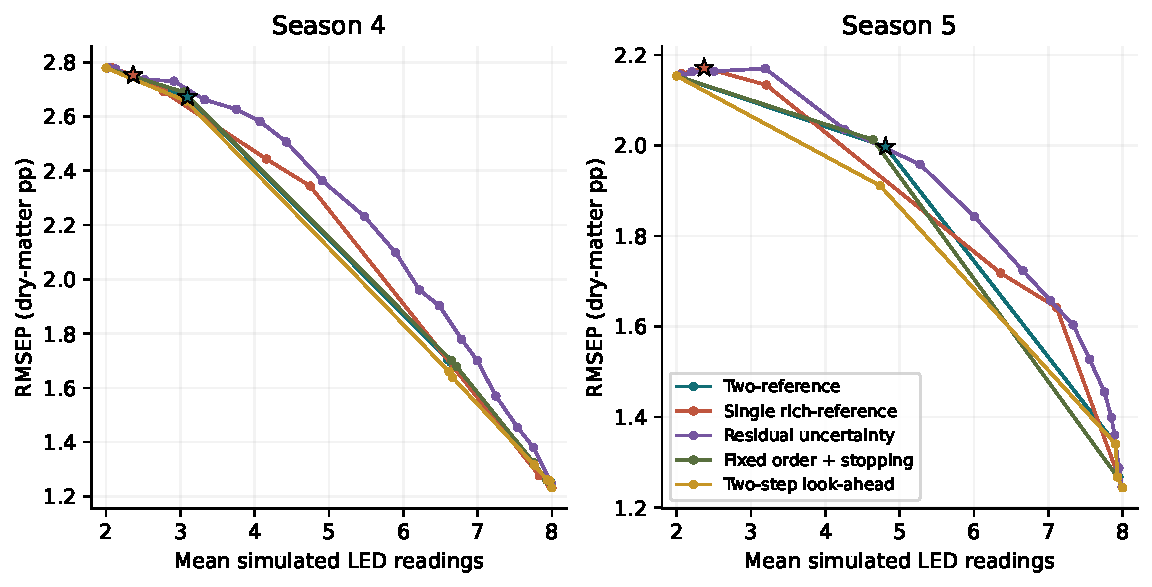
\includegraphics[width=\linewidth]{../figures/error_pulses.pdf}
\caption{Frozen error--acquisition curves, separately by season. Stars mark development-targeted scientific operating points. Curves are descriptive external evaluations, not external optimization.}\label{fig:curves}\end{figure}

\subsection{Mechanism, calibration and limitations of the installed bank}
Table~\ref{tab:mechanism} distinguishes missed corrections among early stops from the complete bank's excess error. Conditional denominators vary with early-exit coverage; comparisons therefore require the accompanying pulse and coverage evidence. Signed gains include both useful and harmful continuations (Figure~\ref{fig:gains}). Reference agreement does not establish small absolute assay error: the exported metrics also retain errors exceeding 2 pp and group-specific results. Visited-state calibration and chosen next-step gain diagnostics are generated separately, without treating multiple states of the same scan as independent fruit.
\begin{table}[tb]\centering\small
\caption{Material corrections and bank losses at $\delta=0.50$ pp. Bank losses are common to policies on the same bank.}\label{tab:mechanism}
\resizebox{\linewidth}{!}{\begin{tabular}{llrrrr}
\toprule
Season & Method & Missed / early & Rate & Early fraction & Bank loss / scans \\
\midrule
4 & Two-reference & 755/1250 & 0.604 & 0.863 & 253/1448 \\
4 & Single-reference & 819/1384 & 0.592 & 0.956 & 253/1448 \\
5 & Two-reference & 106/199 & 0.533 & 0.622 & 9/320 \\
5 & Single-reference & 157/314 & 0.500 & 0.981 & 9/320 \\
\bottomrule
\end{tabular}}
\end{table}
\begin{figure}[tb]\centering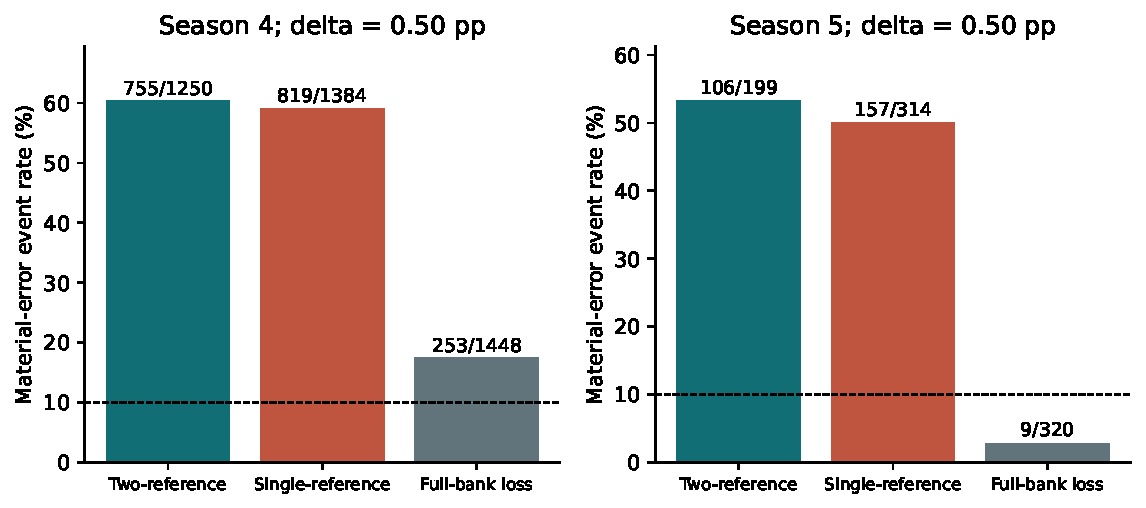
\includegraphics[width=\linewidth]{../figures/missed_and_bank_losses.pdf}
\caption{Missed-correction and bank-loss rates with exact event denominators. Dashed lines show the illustrative 10\% development criterion. External rates do not recalibrate that criterion.}\end{figure}
\begin{figure}[tb]\centering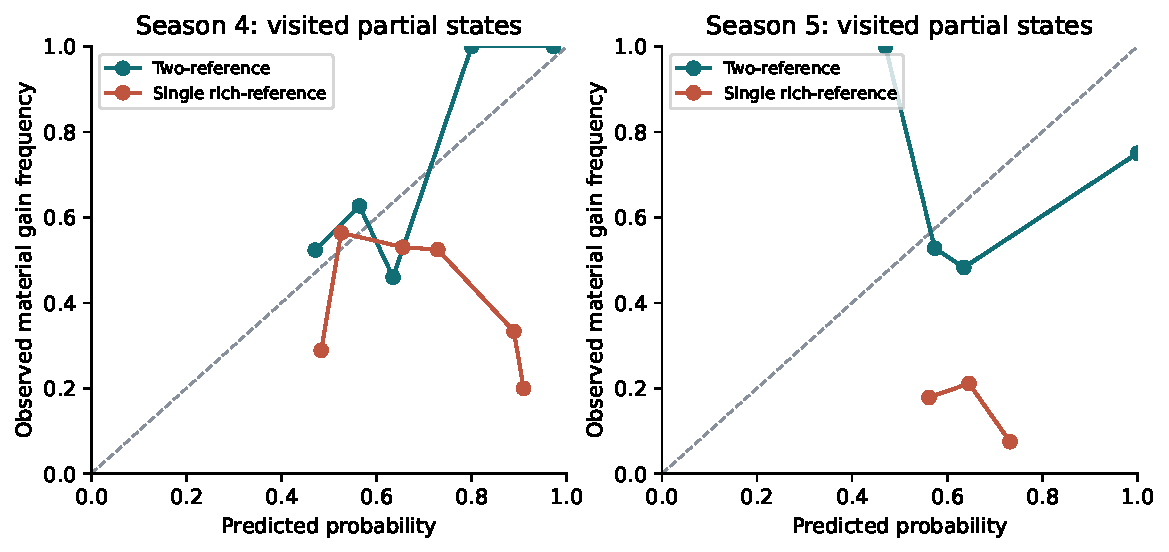
\includegraphics[width=\linewidth]{../figures/calibration.pdf}
\caption{Probability calibration on visited partial states. These state-level diagnostics differ from final stopped-scan outcomes.}\end{figure}
\begin{figure}[tb]\centering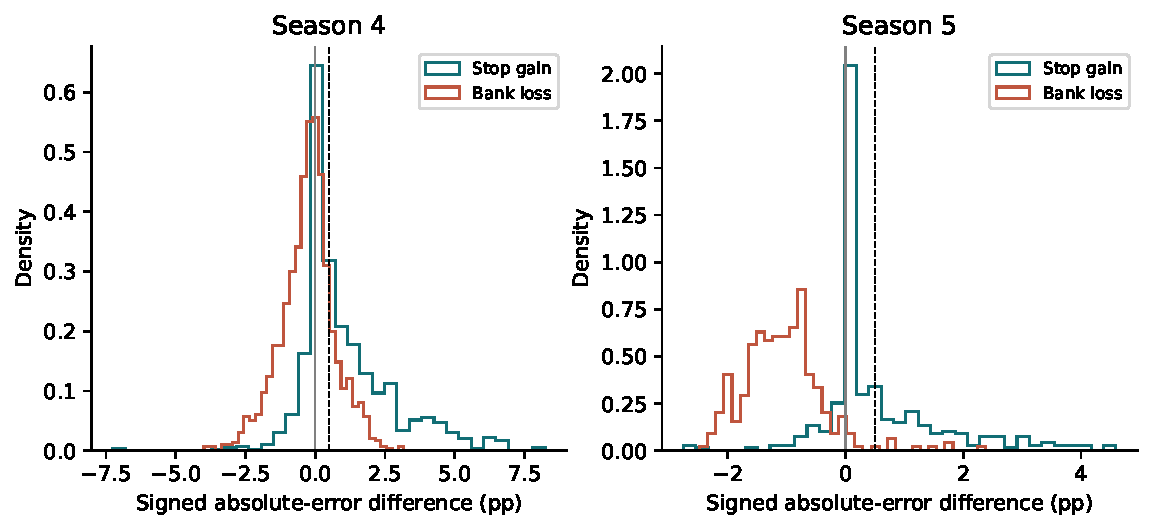
\includegraphics[width=\linewidth]{../figures/signed_gains.pdf}
\caption{Signed stop gains at selected final decisions and bank--rich-reference error gaps. Negative values are retained.}\label{fig:gains}\end{figure}

\section{Discussion}
\subsection{Ordering controls and fixed-budget alternatives}
In season 4, fixed ordering with adaptive stopping achieved 2.690 pp at 3.046 readings, and the two-step look-ahead approximation achieved 2.657 pp at 3.077 readings. In season 5, fixed ordering with adaptive stopping achieved 2.013 pp at 4.641 readings, and the two-step look-ahead approximation achieved 1.911 pp at 4.737 readings. Table~\ref{tab:controls} gives achieved acquisition budgets, which remain essential to interpretation. The supplement contains all static PLSR, SVR and MLP budgets, alternate bank selectors, ideal-point analyses, response shifts and seed comparisons. A better complete-bank regressor using the same channels would indicate that part of the apparent bank limitation is statistical rather than optical.
\begin{table}[tb]\centering\small
\caption{Primary-bank controls and selected fixed-budget physical references, seed 42. Fixed-length scans use their development-selected length.}\label{tab:controls}
\begin{tabular}{llrrr}
\toprule
Season & Control/reference & RMSEP & Readings & Early fraction \\
\midrule
4 & Residual uncertainty & 2.364 & 4.91 & 0.608 \\
4 & Fixed order + stopping & 2.690 & 3.05 & 0.866 \\
4 & Fixed-length scan & 2.851 & 4.00 & 1.000 \\
4 & Random order + stopping & 2.662 & 3.17 & 0.841 \\
4 & Two-step look-ahead & 2.657 & 3.08 & 0.865 \\
4 & physical plsr 4 & 1.242 & 4.00 & 1.000 \\
4 & physical plsr 8 & 1.232 & 8.00 & 0.000 \\
4 & physical sparse svr 4 & 2.361 & 4.00 & 1.000 \\
4 & physical sparse svr 8 & 2.504 & 8.00 & 0.000 \\
5 & Residual uncertainty & 1.657 & 7.03 & 0.275 \\
5 & Fixed order + stopping & 2.013 & 4.64 & 0.650 \\
5 & Fixed-length scan & 2.230 & 4.00 & 1.000 \\
5 & Random order + stopping & 1.828 & 5.10 & 0.562 \\
5 & Two-step look-ahead & 1.911 & 4.74 & 0.631 \\
5 & physical plsr 4 & 1.853 & 4.00 & 1.000 \\
5 & physical plsr 8 & 1.244 & 8.00 & 0.000 \\
5 & physical sparse svr 4 & 1.530 & 4.00 & 1.000 \\
5 & physical sparse svr 8 & 1.604 & 8.00 & 0.000 \\
\bottomrule
\end{tabular}
\end{table}

Season 4 visited-state Brier scores were 0.263 and 0.260 for the two-reference and single-reference targets. The engineering point used 7.942 readings with RMSEP 1.261 pp. Fixed four-LED PLSR and sparse SVR achieved 1.242 and 2.361 pp. Season 5 visited-state Brier scores were 0.270 and 0.346 for the two-reference and single-reference targets. The engineering point used 8.000 readings with RMSEP 1.244 pp. Fixed four-LED PLSR and sparse SVR achieved 1.853 and 1.530 pp.
The Brier scores concern different target events and visited states, so their values are diagnostics rather than a direct ranking of stopping objectives. The engineering point largely reads the complete bank; the scientific point saves readings at excessive assay error. Fixed-order differences are descriptively small, while the fixed-budget regressors expose substantial partial-prediction error. The results do not establish value for the additional adaptive-controller complexity. Simpler fixed acquisition and improved calibration are priorities for a new development study.

The illustrative prototype criteria did not hold in both seasons. A lower policy RMSEP at a different acquisition budget does not isolate the value of the objective. The frozen curves, same-bank single-reference contrast, independent-bank sensitivity and stopping/order controls are needed together. When fixed order offers a comparable trade-off, a simpler controller is preferable. When the complete bank remains substantially less accurate than the rich reference, changing stopping logic cannot recover missing optical information; optical coverage and transfer should be investigated first.

The empirical interpretation is constrained by reused public seasons, unavailable fruit identifiers, a season represented by only two populations, and the simulated measurement model. Bank-loss differences also reflect model-fitting choices. Typical emitter plots, assumed detector response and conventional log-base interpretation need direct optical validation. Calibration on training seasons does not confer distribution-free risk control under later-season shift. The bounded search and compact models are reproducible alternatives, not proof that the best possible scanner or baseline has been found. Inaccessible prior methods remain a limit on novelty assessment.

An appropriate physical follow-up would acquire adaptive and fixed scans on the same newly collected fruits, obtain oven-dry reference values, measure emission and detector responses, energy per scan, time and placement repeatability, and evaluate a genuinely later harvest. No patentability conclusion follows from the paper-level prior-art comparison.

\section{Software, data and declarations}
The offline application and CLI load the same frozen bank and model. A \texttt{read\_channel(led\_id)} boundary reveals only the requested reading. The distributed real development example omits its assay; manual mode requires neither a full spectrum nor a CSV. The executable workflow supports smoke checks, resumable execution, verification, replay, the local app and reporting-only regeneration. A deliberate interruption was recovered without changing completed checkpoint hashes. The original data are available under CC BY 4.0 at the versioned DOI; local artifacts include exact provenance and hashes. No public repository release or manuscript submission occurred in this run.

Author input required: author names, affiliations, author contributions, funding, competing interests, and any institution-specific declaration wording. The study reuses public mango research data and does not report new human or animal experiments. These fields must be confirmed by the authors before submission.

\clearpage
\bibliographystyle{plainnat}
\bibliography{references}
\end{document}
